
\addcontentsline{toc}{section}{Introduction}
\section{Introduction}
L'objectif de cette partie est de présenter le contexte général du projet, en commençant par l'organisme d'accueil, IZICAP, où je suis en train d'effectuer un stage de 5 mois. Nous décrirons leurs activités, leur stratégie, leurs valeurs, ainsi que l'organigramme et les profils impliqués dans mon projet. Ensuite, nous aborderons la demande de travaux qui exprime les besoins fonctionnels sur lesquels je me suis basé pour concevoir et réaliser la solution, ainsi que la méthodologie suivie pour atteindre les objectifs fixés.

\section{Présentation de l’organisme d’accueil}
\subsection{IZICAP}
IZICAP est une société unique et novatrice axée sur l'analyse de données, la fidélisation et le marketing numérique pour les petites et moyennes entreprises (PME). Leur solution conviviale et facile à installer repose sur le modèle SaaS, permettant d'exploiter les données transactionnelles des cartes de paiement des clients.

En collaborant avec les banques et les acquéreurs, IZICAP offre une proposition de valeur renforcée et mettons à leur disposition un outil puissant de marketing numérique destiné aux PME. Leur mission est d'accompagner les commerçants au quotidien pour accélérer le développement de leur entreprise, répondant ainsi à leurs besoins spécifiques.

L'histoire d'IZICAP remonte à 2013, lorsque elle a vu le jour dans un paysage des services financiers en constante évolution et de plus en plus complexe. Depuis lors, les modèles bancaires et de paiement traditionnels sont continuellement menacés par de nouvelles entreprises challengers plus innovantes. Une concurrence agressive signifie que la fidélité des commerçants ne peut plus être considérée comme acquise, et souvent les acquéreurs et les fournisseurs de services de paiement sont contraints de réduire leurs frais.

Après s'être solidement implantée en France grâce à des partenariats avec le Groupe BPCE et le Crédit Agricole, Izicap a établi un partenariat avec Nexi, le principal acquéreur et fintech en Italie, et a rejoint le programme StartPath de Mastercard dans le but d'étendre considérablement sa portée à l'échelle mondiale. Cette expansion stratégique renforce Leur position sur le marché et confirme Leur engagement à offrir leur services à un public plus large.

Avec Izicap, les PME ont accès à une solution innovante qui tire parti de l'analyse de données pour optimiser leur stratégie de fidélisation et de marketing. Grâce à leur expertise et à leur présence internationale croissante, IZICAP est déterminée à soutenir la croissance des entreprises et à les aider à prospérer dans un environnement commercial en constante évolution.

\cite{izicap}

\subsection{Partenariats stratégiques}
IZICAP a établi des partenariats stratégiques avec plusieurs acteurs clés de l'industrie financière. Parmi ses partenaires notables figurent :
\begin{itemize}
    \item \textbf{Groupe BPCE:} Izicap a collaboré avec le Groupe BPCE, l'un des principaux groupes bancaires en France, pour fournir sa solution de fidélisation et de marketing numérique aux commerçants.
    \item \textbf{Crédit Agricole:} Izicap a établi un partenariat avec Crédit Agricole, l'une des plus grandes banques françaises, afin d'offrir ses services aux commerçants de leur réseau.
    \item \textbf{Nexi:} Izicap a noué un partenariat avec Nexi, le principal acquéreur et fintech en Italie. Cette collaboration permet à Izicap d'étendre sa présence sur le marché italien et de bénéficier de l'expertise de Nexi dans le domaine des services de paiement.
    \item \textbf{Mastercard StartPath:} Izicap a rejoint le programme StartPath de Mastercard, qui soutient les start-ups et les entreprises innovantes dans le domaine des technologies financières. Cette collaboration offre à Izicap l'opportunité d'accroître sa visibilité et son expansion internationale.
    \item \textbf{BBVA:} Izicap a également établi un partenariat avec BBVA, l'une des principales banques en Espagne et en Amérique latine. Cette collaboration avec BBVA renforce la présence d'Izicap sur le marché espagnol et permet à la société d'offrir ses solutions de fidélisation et de marketing numérique aux commerçants affiliés à BBVA. Le partenariat avec BBVA témoigne de l'engagement d'Izicap à étendre sa portée et à travailler avec des acteurs majeurs de l'industrie financière pour soutenir les petites et moyennes entreprises dans leur croissance.
    \item \textbf{Ingenico:} Izicap a établi un partenariat avec Ingenico, l'un des principaux fournisseurs de solutions de paiement et de services marchands au niveau mondial. Grâce à ce partenariat, Izicap est en mesure d'intégrer sa solution de fidélisation et de marketing numérique aux terminaux de paiement d'Ingenico, offrant ainsi une solution complète aux commerçants utilisant les services d'Ingenico. Cette collaboration renforce la position d'Izicap en tant que fournisseur de solutions de fidélisation et de marketing innovantes, en s'appuyant sur l'expertise et la portée mondiale d'Ingenico dans le secteur des paiements.
\end{itemize}
\begin{figure}[H]
\centering

\includegraphics[width=\linewidth]{images/partenaires.png}
\caption{Partenariats stratégiques}\label{fig:partenaires}
\end{figure}    
\section{Organigramme}
\begin{figure}[H]
\centering
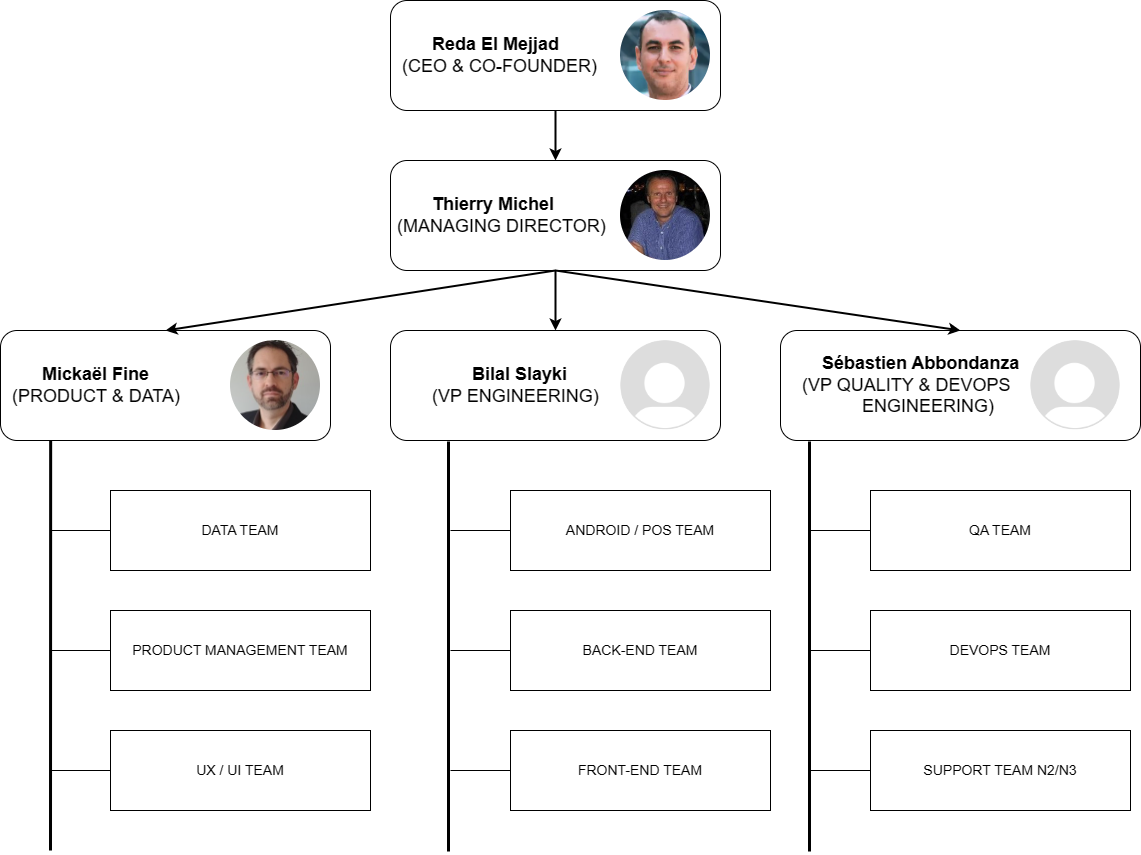
\includegraphics[width=0.75\linewidth]{images/organigram.png}
\caption{Organigramme de Izicap}\label{fig:organigmramme}
\end{figure}

Au sein de l'équipe de projet, j'ai eu l'opportunité de travailler de manière polyvalente dans différents domaines. J'ai contribué activement au développement du backend en participant à la conception et à l'implémentation des microservices. J'ai également collaboré avec l'équipe frontend en apportant mon expertise pour l'intégration des microfrontends et l'amélioration de l'expérience utilisateur. De plus, j'ai été impliqué dans la gestion des données en participant à la mise en place de Delta Lake et en contribuant à l'optimisation des flux de données. Cette expérience diversifiée m'a permis d'acquérir une vision globale du projet et de collaborer efficacement avec différentes équipes pour atteindre les objectifs fixés.

\section{Cadre du projet}

Le projet consiste à refonter l'application `Smart data' qui fait référence au processus d'extraction d'informations précieuses à partir de grandes quantités de données afin de prendre des décisions commerciales éclairées.

La smart data nous permet de:

\begin{enumerate}
    \item \textbf{Collecte des données}: Izicap aide les entreprises à collecter des données clients à partir de différents points de contact tels que les systèmes de point de vente, les programmes de fidélité, les interactions en ligne, etc. Assurez-vous d'intégrer leurs outils de collecte de données dans vos systèmes ou processus existants.
    \item \textbf{Analyse des données}: La solution de smart data d'Izicap vous permet d'analyser les données collectées pour découvrir des tendances, des modèles et des comportements clients. Utilisez leurs outils d'analyse et leurs algorithmes pour obtenir des informations exploitables à partir des données.
    \item \textbf{Segmentation des clients}: Segmentez votre base de clients en fonction de leurs préférences, de leur historique d'achat, de leurs caractéristiques démographiques ou d'autres critères pertinents. La solution de smart data d'Izicap peut vous aider à identifier différents segments de clients et à créer des stratégies marketing personnalisées pour chaque segment.
    \item \textbf{Marketing personnalisé}: Exploitez les informations tirées de la solution de smart data d'Izicap pour créer des campagnes marketing ciblées. Envoyez des offres personnalisées, des promotions ou des recommandations à des segments spécifiques de clients, augmentant ainsi les chances de conversion et de satisfaction client.
    \item \textbf{Fidélisation de la clientèle}: Utilisez la solution de smart data d'Izicap pour identifier les clients qui risquent de résilier leur abonnement ou de ne plus acheter chez vous. Développez des stratégies de fidélisation en leur offrant des incitations, des programmes de fidélité ou des communications personnalisées afin de les maintenir engagés et fidèles à votre marque.
    \item \textbf{Suivi des performances}: Surveillez régulièrement les performances de vos campagnes marketing et de vos efforts d'engagement client. La solution d'Izicap peut vous fournir des métriques et des rapports pour évaluer l'efficacité de vos stratégies et apporter des ajustements basés sur les données lorsque nécessaire.
    \item \textbf{Amélioration continue}: Les solutions de smart data sont les plus efficaces lorsqu'elles sont utilisées de manière itérative. Analysez régulièrement les données, adaptez vos stratégies et peaufinez votre approche en fonction de nouvelles informations et de l'évolution du comportement client.
\end{enumerate}


\begin{figure}[H]
\centering
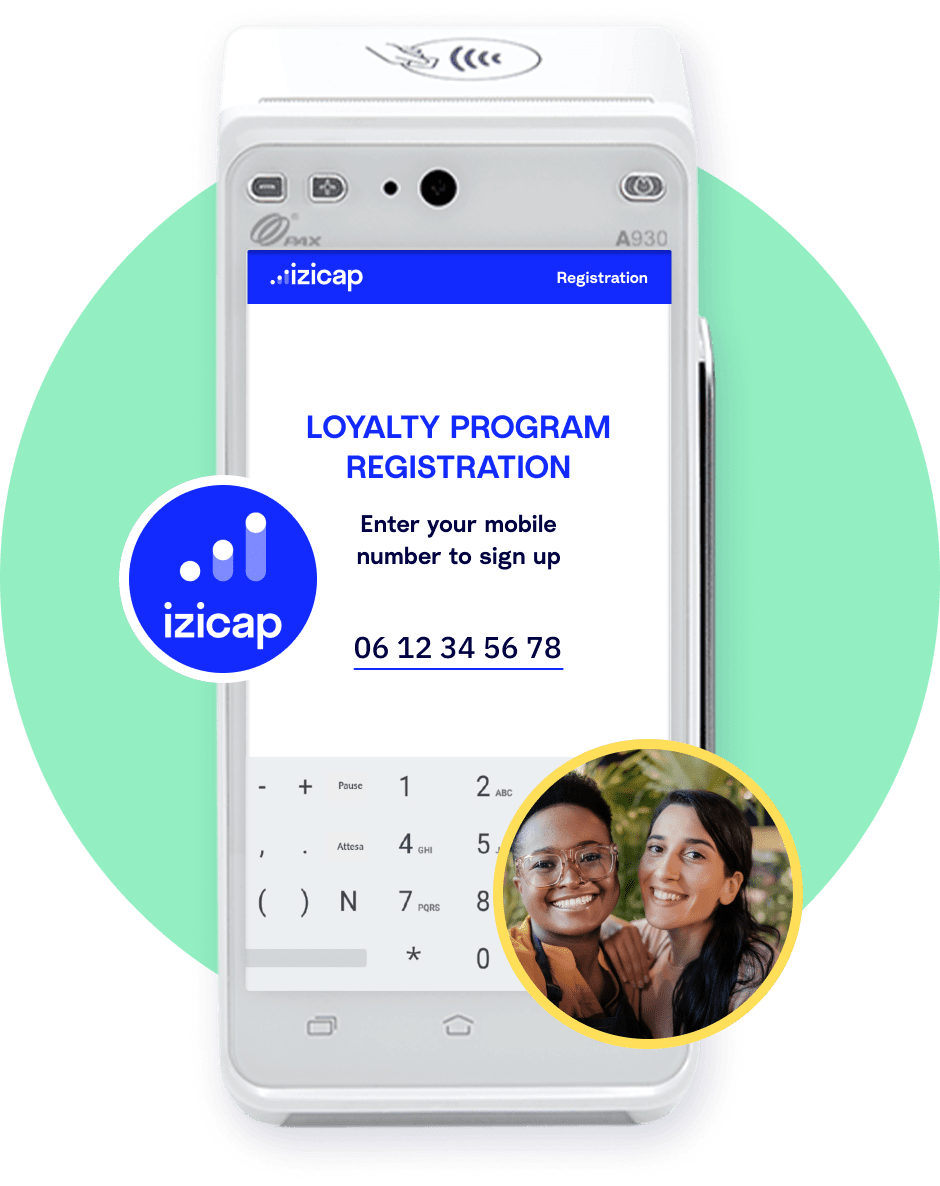
\includegraphics[width=0.6\linewidth]{images/smart-data-izicap.png}
\caption{Smart data Izicap}\label{fig:smart-data-Izicap}
\end{figure}


\section{L'architecture du système -Smart Data-}

La figure ci-dessous visualise la structure et les composants clés de notre système, ainsi que les interactions entre eux, elle constitue ainsi le fondement de notre système et joue un rôle essentiel dans la fourniture de fonctionnalités et de services à nos utilisateurs.

\begin{figure}[H]
\centering
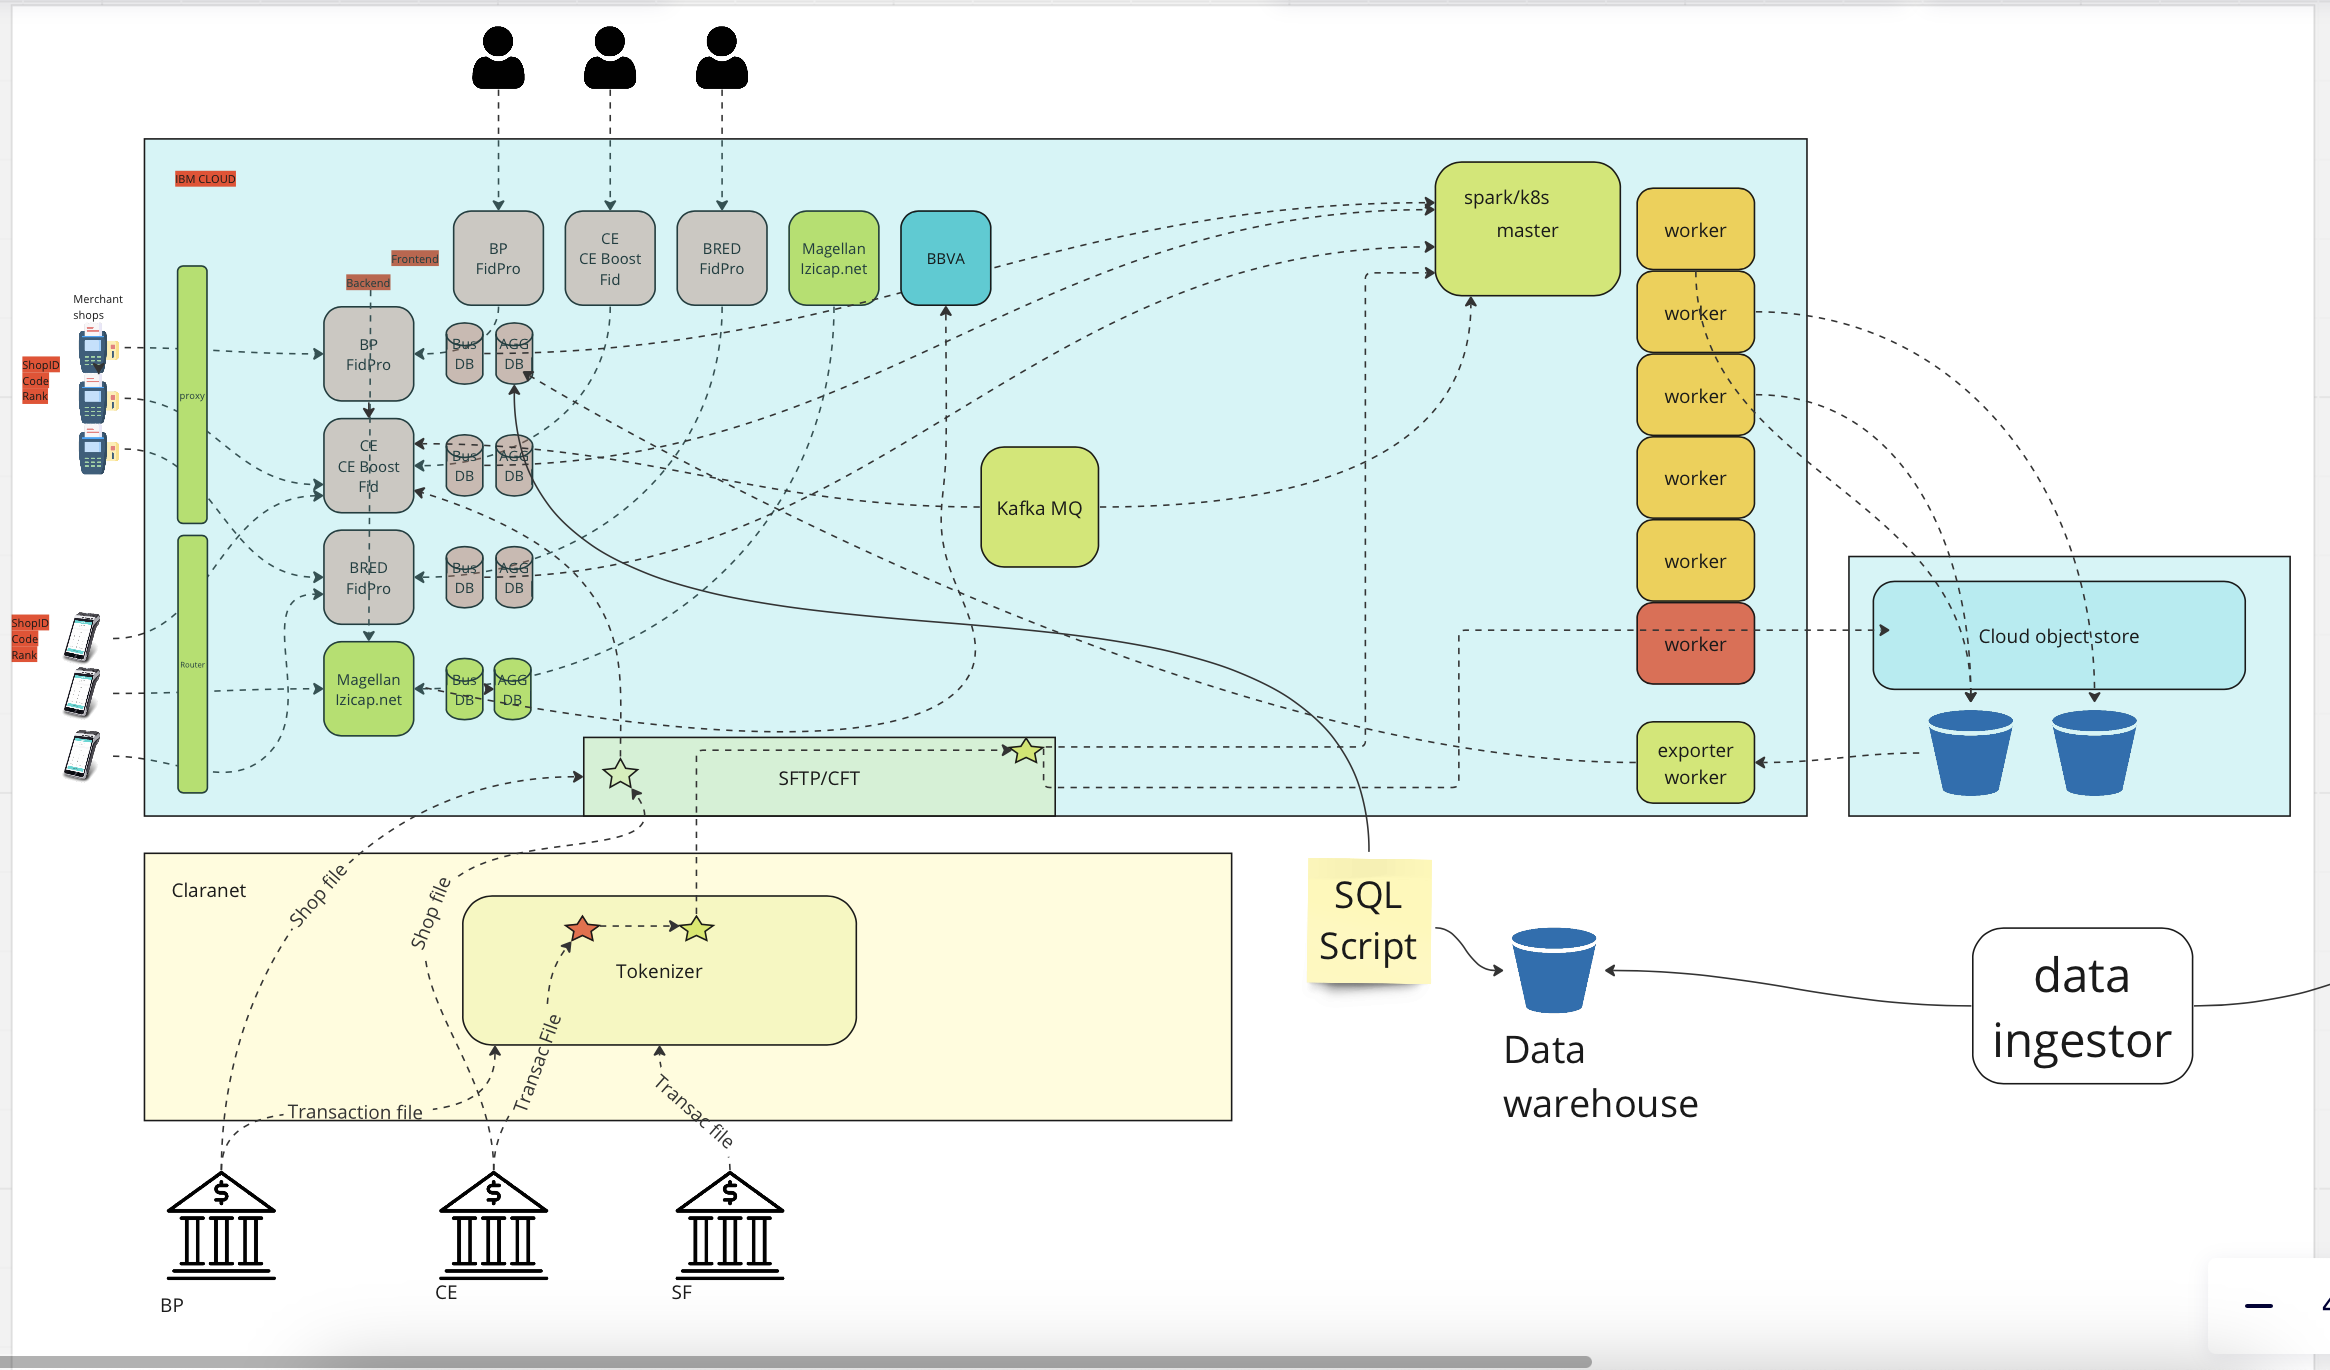
\includegraphics[width=\linewidth]{images/archi-globale.png}
\caption{Architecture du système actuelle}\label{fig:architecture-monolithique}
\end{figure}

Ce schéma représente le fonctionnement de l'architecture monolithique actuelle qui présente plusieurs inconvénients qui peuvent entraver l'efficacité, la flexibilité et la maintenabilité du système. Voici une description détaillée des principaux inconvénients:

\begin{enumerate}
    \item \textbf{Complexité et dépendances}: L'architecture monolithique implique que tous les modules et fonctionnalités du système sont regroupés en un seul bloc. Cela crée une forte interdépendance entre les différents composants, rendant la compréhension, la gestion et les mises à jour complexes. Les modifications apportées à une partie du système peuvent avoir des répercussions sur d'autres parties, ce qui rend les tests, les déploiements et les corrections d'erreurs plus difficiles.
    \item \textbf{Scalabilité limitée}: L'architecture monolithique a souvent des difficultés à s'adapter à une augmentation de la charge ou à une demande croissante. Étant donné que tous les composants sont regroupés dans un seul monolithe, il est difficile de faire évoluer sélectivement une partie spécifique du système. Cela peut entraîner des goulots d'étranglement, des performances réduites et une mauvaise répartition des ressources lorsqu'il s'agit de traiter des volumes de données importants ou de gérer une augmentation du nombre d'utilisateurs.
    \item \textbf{Déploiements complexes et risques élevés}: Avec une architecture monolithique, les déploiements nécessitent la mise à jour de l'ensemble du système, même pour des modifications mineures. Cela augmente les risques d'erreurs et de régressions, car une seule erreur peut entraîner l'indisponibilité du système tout entier. De plus, les déploiements doivent être soigneusement planifiés et coordonnés, ce qui peut entraîner des temps d'arrêt plus longs et des interruptions de service pour les utilisateurs.
    \item \textbf{Difficulté de choix technologiques}: Dans une architecture monolithique, les technologies utilisées sont souvent liées et intégrées de manière étroite. Cela peut rendre difficile l'adoption de nouvelles technologies ou l'intégration de composants spécialisés. Les mises à niveau de versions ou les ajouts de nouvelles fonctionnalités peuvent être limités par les choix technologiques initiaux, ce qui peut entraver l'innovation et l'adaptation aux évolutions du marché.
    \item \textbf{Cohésion et responsabilités}: L'architecture monolithique ne facilite pas une séparation claire des responsabilités et des fonctionnalités. Les différents modules du système sont souvent intimement liés et peuvent partager des fonctionnalités communes. Cela rend difficile l'isolation des problèmes, la maintenance spécifique des modules et la réutilisation de code spécifique à un domaine.
\end{enumerate}

\section{Problématique et besoin fonctionnel}
La problématique qui se pose réside dans l'architecture monolithique actuellement utilisée, laquelle présente des limitations en termes de scalabilité, de flexibilité et de maintenabilité. Les contraintes imposées par cette architecture rendent complexe le déploiement de nouvelles fonctionnalités et entraînent des perturbations potentielles dans l'ensemble du système. De plus, l'utilisation d'une base de données relationnelle traditionnelle, telle que MariaDB, se révèle insuffisante pour traiter efficacement de grands volumes de données transactionnelles, il convient de souligner que l'application Smart Data existe depuis maintenant 10 ans et a été développée en utilisant le langage Groovy. Cette longue période d'existence témoigne de la stabilité et de la maturité de notre système. Cependant, l'utilisation du langage Groovy peut présenter certaines contraintes en termes de maintenabilité et d'évolutivité, notamment lorsqu'il s'agit d'intégrer de nouvelles technologies et de gérer des architectures plus modernes.
 
\subsection*{Besoin fonctionnel:}

Afin de répondre à ces problématiques, différents besoins fonctionnels ont été identifiés :

\begin{enumerate}
    \item[$\bullet$] \textbf{Scalabilité}: Il est nécessaire de disposer d'une architecture qui puisse s'adapter facilement à une croissance du nombre d'utilisateurs, des transactions et des données. Il est essentiel que notre système puisse évoluer harmonieusement et maintenir ses performances, même face à une augmentation significative de la charge de travail.
    \item[$\bullet$] \textbf{Flexibilité}: Nous devons être en mesure d'introduire de nouvelles fonctionnalités de manière indépendante et de les déployer sans perturber l'ensemble du système. Une approche basée sur des microservices et des microfrontends nous permettra d'atteindre cette flexibilité, en facilitant le développement, les tests et le déploiement isolé de chaque composant.
    \item[$\bullet$] \textbf{Performances améliorées}: Il est primordial de disposer d'une infrastructure de données capable de gérer efficacement d'importants volumes de données transactionnelles. En remplaçant MariaDB par Delta Lake, nous pourrons tirer parti de fonctionnalités avancées telles que la gestion des transactions ACID et la compatibilité avec des outils d'analyse performants, ce qui améliorera sensiblement les performances et la fiabilité de notre système.
    \item[$\bullet$] \textbf{Séparation des responsabilités}: Nous visons une meilleure séparation des responsabilités entre les différents composants de notre système. Les microservices nous permettront de découpler les fonctionnalités, de les attribuer à des équipes spécifiques et de favoriser une gestion du code plus efficace, une maintenance simplifiée et une évolutivité accrue.
\end{enumerate}


\section{Objectives du stages}
Le projet s'inscrit dans le cadre du renouvellement des fonctionnalités de l'application Smart Data, visant à améliorer sa scalabilité, sa flexibilité et ses performances. Dans ce contexte, les objectifs du stage sont les suivants :

\begin{enumerate}
    \item Étudier et analyser l'architecture actuelle de l'application SMART DATA afin de comprendre les contraintes et les limitations qui entravent sa croissance et son évolution.
    \item Proposer et concevoir une stratégie de migration de l'architecture monolithique vers une architecture basée sur des microservices et des microfrontends, permettant ainsi une meilleure modularité et une plus grande flexibilité dans le développement et le déploiement des fonctionnalités.
    \item Mettre en œuvre multiples microservices avec Springboot dans le cadre de la nouvelle architecture, en utilisant une technologie appropriée et en veillant à son intégration harmonieuse avec les autres composants du système.
    \item Évaluer les avantages et les implications de l'utilisation de Delta Lake en remplacement de la base de données MariaDB, en mettant l'accent sur les performances, la gestion des transactions et l'intégration avec les outils d'analyse.
    \item Intégrer Trino dans l'architecture pour permettre l'exécution de requêtes SQL complexes et optimiser le traitement des données, en assurant une collaboration efficace avec l'équipe de développement.
    \item Mettre en place une infrastructure de déploiement et de gestion des microservices, en utilisant des outils tels que Kubernetes, Docker et Jenkins, pour faciliter le déploiement, la mise à l'échelle et la gestion des composants.
    \item Concevoir et mettre en œuvre des tests unitaires et des tests d'intégration pour assurer la qualité et la fiabilité des nouveaux composants développés dans le cadre de l'architecture basée sur les microservices.
    \item Documenter de manière approfondie le processus de migration et les choix technologiques effectués, fournissant des instructions claires pour la maintenance future de l'architecture et la gestion des mises à jour.
    \item Collaborer étroitement avec l'équipe existante pour faciliter la transition vers la nouvelle architecture, en offrant un soutien technique, des conseils et des formations sur les nouvelles technologies utilisées.
\end{enumerate}

\section{Processus de réalisation du projet}

Le processus de réalisation du projet s'est déroulé en plusieurs itérations appelées `sprints', d'une durée généralement fixe de deux semaines. Chaque sprint était axé sur la livraison d'incréments fonctionnels de l'application, permettant ainsi d'obtenir rapidement des résultats tangibles.

Voici les étapes clés du processus de réalisation du projet, basé sur la méthodologie Scrum:

\begin{enumerate}
    \item \textbf{Définition du backlog du produit:} En collaboration avec les parties prenantes et l'équipe de développement, nous avons identifié et priorisé les fonctionnalités à développer et à intégrer dans l'architecture basée sur les microservices.
    \item \textbf{Planification du sprint:} Au début de chaque sprint, nous avons organisé une réunion de planification pour définir les objectifs spécifiques du sprint, sélectionner les tâches à réaliser et estimer les efforts nécessaires.
    \item \textbf{Développement itératif:} L'équipe de développement a travaillé de manière itérative sur les tâches assignées, en se concentrant sur la réalisation des fonctionnalités identifiées pour le sprint en cours.
    \item \textbf{Réunions quotidiennes de stand up:} Chaque jour, l'équipe s'est réunie pour une brève réunion de stand-up afin de partager les progrès, les obstacles éventuels et coordonner les activités.
    \item \textbf{Revue de sprint:} À la fin de chaque sprint, nous avons organisé une revue de sprint pour présenter les fonctionnalités développées et obtenir des retours des parties prenantes. Cela nous a permis de valider les résultats obtenus et de planifier les prochaines étapes.
    \item \textbf{Rétrospective de sprint:} Après la revue de sprint, nous avons mené une rétrospective pour évaluer le déroulement du sprint, identifier les points forts et les points à améliorer, et ajuster notre approche en conséquence.
    \item \textbf{Itérations suivantes:} Le processus de planification, de développement itératif, de revue de sprint et de rétrospective s'est répété pour chaque sprint suivant, permettant ainsi une progression incrémentale vers les objectifs du projet.
\end{enumerate}

\begin{figure}[H]
\centering
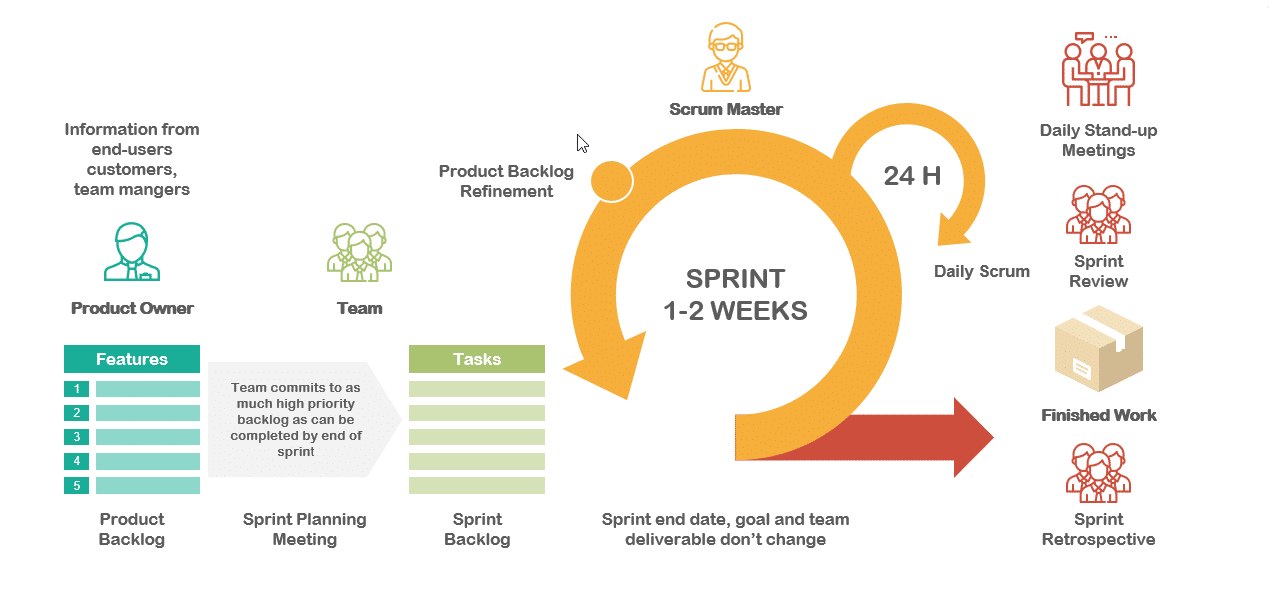
\includegraphics[width=\linewidth]{images/scrum.png}
\caption{Méthodologie Scrum}\label{fig:scrum}
\end{figure}

\section{Planification du projet}
Pour la planification du projet, nous avons utilisé la méthode de modélisation du réseau de dépendance entre les tâches. Cette approche nous a permis de décomposer le travail en différentes tâches structurées et d'établir des relations de dépendance entre elles.

Nous avons également utilisé la technique du diagramme de Gantt pour représenter graphiquement les tâches et les ressources du projet dans le temps. En ligne, nous avons listé les différentes tâches, et en colonne, nous avons défini les jours, les semaines ou les mois. Chaque tâche a été représentée par une barre dont la longueur est proportionnelle à la durée estimée de cette tâche.

Le diagramme de Gantt nous a permis de visualiser la répartition des tâches, leur durée et leur succession. Certaines tâches se sont réalisées en séquence, tandis que d'autres ont pu être réalisées en parallèle, de manière partielle ou totale. Cette représentation claire et visuelle nous a aidés à planifier le projet en déterminant et en organisant les différentes tâches de manière à assurer une gestion efficace du projet.

La figure suivante présente le diagramme de Gantt détaillant la planification du projet, avec les tâches ordonnées dans le temps et leur durée respective. Cela nous a permis de suivre l'avancement du projet, d'identifier les éventuels retards et de prendre les mesures appropriées pour les résoudre.

\begin{figure}[H]
\centering
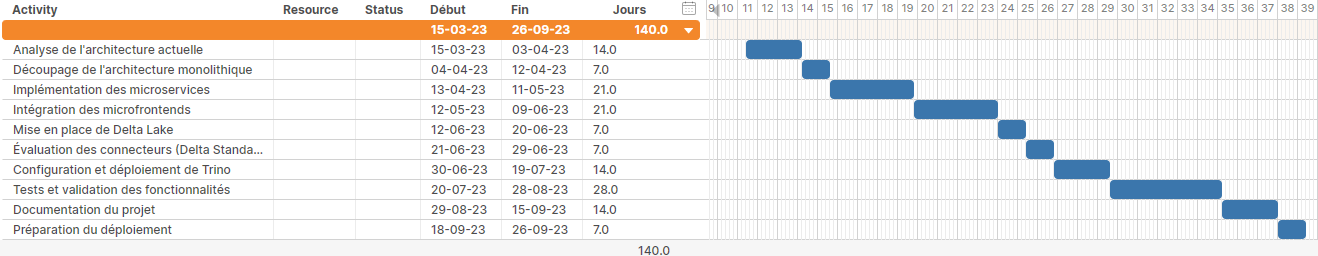
\includegraphics[width=\linewidth]{images/gantt.png}
\caption{Diagramme de Gantt}\label{fig:gantt}
\end{figure}

\addcontentsline{toc}{section}{Conclusion}
\section*{Conclusion}

En conclusion de cette section, nous avons présenté la planification du projet de renouvellement des fonctionnalités de l'application SMART DATA. Nous avons élaboré un planning basé sur la modélisation du réseau de dépendance entre les tâches, en utilisant la technique du diagramme de Gantt. Ce diagramme nous a permis de visualiser les différentes activités, leur durée estimée et les ressources nécessaires.

Au cours de la planification, nous avons identifié les principales activités du projet, telles que l'analyse de l'architecture actuelle, le découpage de l'architecture monolithique, l'implémentation des microservices, l'intégration des microfrontends, la mise en place de Delta Lake, l'évaluation des connecteurs, la configuration et le déploiement de Trino, les tests et la validation des fonctionnalités, la documentation du projet, la préparation du déploiement, ainsi que la formation et la sensibilisation des utilisateurs.

Nous avons également pris en compte la durée totale du projet, qui est estimée à 5 mois, et avons ajusté les durées des activités en conséquence. Cela nous a permis d'avoir une vision plus précise de la planification temporelle du projet.